\documentclass[a4paper,12pt]{scrreprt}
\usepackage[within=none]{caption}
% Für deutsche Überschriften, usw. dieses Paket aktivieren
% \usepackage[ngerman]{babel}

%% REQUIRED PACKAGES
\usepackage{amsfonts,amsmath,amssymb} % math stuff
\usepackage{booktabs} % better layout for tables
\usepackage{color} % enable use of colors
\usepackage{fancyhdr} % definition of own headers/footers
\usepackage{graphicx} % for including pictures
\usepackage{units} % for giving quantities the right surrounding
\usepackage{xspace} % correct spacing behind DuMuX command
\usepackage{here} %to force graphic to be exactly HERE
\usepackage{epstopdf} %to include eps 


%% OPTIONAL PACKAGES
\usepackage{array,caption} % needed for the new column type
\usepackage{lipsum} % dummy text with \lipsum[1]
\usepackage{subcaption} % multiple figures in one row
\usepackage{rotating} % rotating of figures
\usepackage{listings}
\lstset{inputpath=../../}
\usepackage{chngcntr}
\counterwithout{equation}{chapter}
\usepackage[shortlabels]{enumitem}
\setlist[enumerate]{noitemsep}

\usepackage[bookmarks=true,bookmarksopen=true,bookmarksopenlevel=2]{hyperref} % enable links
\hypersetup{
%  pdfpagemode=None,
  pdfpagemode=UseOutlines,
  pdfstartview=Fit,
  pdftitle={},
  pdfsubject={},
  pdfauthor={},
  pdfkeywords={},
  pdfcreator={pdflatex}
}

%\usepackage{todonotes} % for colorful todo notes
\usepackage[disable]{todonotes} % for colorful todo notes
\usepackage{trackchanges}

%% PAGE SETUP
\textheight 22.5cm
\textwidth 15.5cm
\oddsidemargin 0.5cm
\evensidemargin 0.5cm
\parindent 0cm
\topmargin 0cm

%% NUMERATION OF ELEMENTS
\setcounter{secnumdepth}{5} % depth of numeration, including \subparagraph
%\renewcommand{\theequation}{\thechapter.\arabic{equation}} % numeration for equations
%\numberwithin{equation}{chapter}
%\renewcommand{\thefigure}{\thechapter.\arabic{figure}} % numeration for figures
%\numberwithin{figure}{chapter}
%\renewcommand{\thetable}{\thechapter.\arabic{table}} % numeration for tables
%\numberwithin{table}{chapter}

%% TEXT APPEARANCE
\renewcommand{\labelitemi}{$-$} % char for itemize environments
\renewcommand{\baselinestretch}{1.05} % line spacing

%% USER DEFINED SETUP
\newcolumntype{V}[1]{>{\raggedright\hspace{0pt}}p{#1}} % columntype with word wrap
\graphicspath{{./Figs/}}
\newcommand{\DuMuX}{DuMu$^\textrm{x}$\xspace}

\definecolor{codegreen}{rgb}{0,0.6,0}
\definecolor{codegray}{rgb}{0.5,0.5,0.5}
\definecolor{codepurple}{rgb}{0.58,0,0.82}
\definecolor{backcolour}{rgb}{0.95,0.95,0.92} 

\lstdefinestyle{mystyle}{
    backgroundcolor=\color{backcolour},
    commentstyle=\color{codegreen},
    keywordstyle=\color{magenta},
    numberstyle=\tiny\color{codegray},
    stringstyle=\color{codepurple},
    basicstyle=\footnotesize,
    breakatwhitespace=false,
    breaklines=true,
    captionpos=b,
    keepspaces=true,
    numbers=left,
    numbersep=5pt,
    showspaces=false,
    showstringspaces=false,
    showtabs=false,
    tabsize=2
} 

\lstset{language={C++},
style=mystyle,
breaklines=true,
frame=single}

\title{The new version of DuMu$^x$ including the modules ``CRootBox" and ``dumux-rosi"}
\subtitle{Documentation}

\author{Manual written by A. Schnepf}
\date{\today} 

\begin{document}

\maketitle

%\begin{figure}[ht]
	%\centering
  %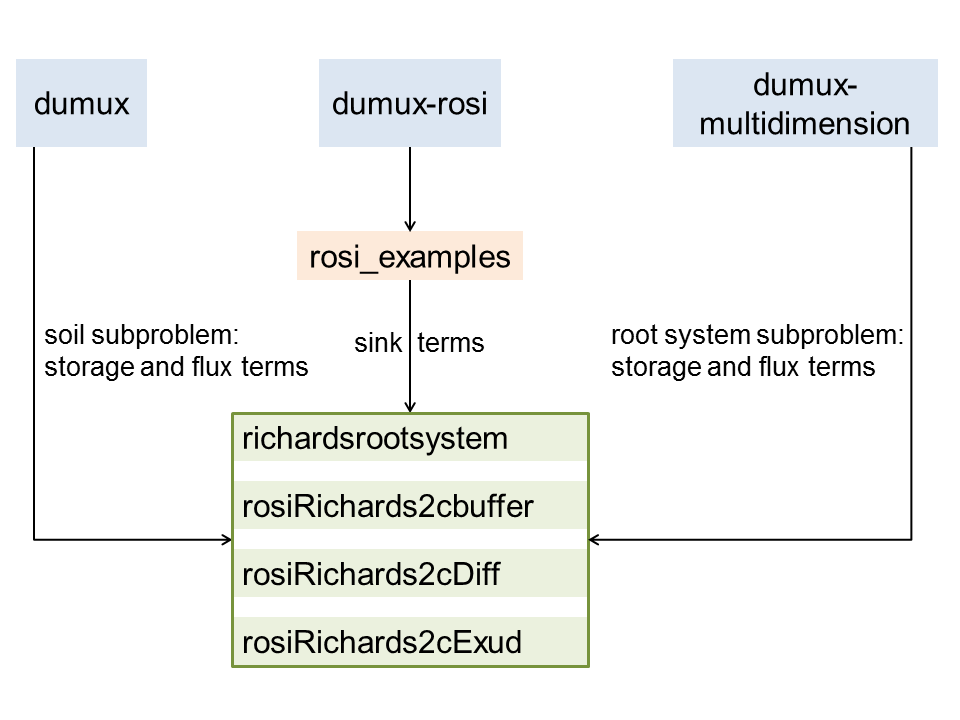
\includegraphics[width=0.9\textwidth]{Overview.png}
	%\captionsetup{labelformat=empty}
	%\caption{Overview of the link between CRootBox and DuMu$^x$}
	%\label{Overview}
%\end{figure}

\chapter*{Installation}
This installation guidelines are for the new version of DuMu$^{x}$, version 3, coupled with CRootBox, in Linux systems (e.g. Ubuntu). 

\section*{Required compilers and tools}
%
If on a recent Ubuntu system, the c++ compiler and python that come with the distribution are recent enough. Otherwise, please make sure you have a recent c++ compiler (e.g. \lstinline{sudo apt-get install clang}) and python3 (e.g. \lstinline{sudo apt-get install python3.6}). 

- Install git: \\
\lstinline{sudo apt-get install git}\\
- Install cmake:\\
\lstinline{sudo apt-get install cmake}\\
- Install libboost:\\
\lstinline{sudo apt-get install libboost-all-dev}\\
- Install pip:\\
\lstinline{sudo apt-get install python3-pip}\\
- Install the python package numpy:\\
\lstinline{pip3 install numpy}\\
- Install the python package scipy:\\
\lstinline{pip3 install scipy}\\
- Install the python package matplotlib:\\
\lstinline{pip3 install matplotlib}\\
- Install the java runtime environment:\\
\lstinline{sudo apt-get install default-jre}\\
- Install Paraview\\
\lstinline{sudo apt-get install paraview}\\


\lstinline{}\\

\section*{DuMu$^x$ installation}
In all dune modules we stay in version 2.6, the latest stable release version. 

- Create a DUMUX folder\\
\lstinline{mkdir DUMUX}\\
\lstinline{cd DUMUX}\\
- Download DUNE core modules:\\
\texttt{git clone https://gitlab.dune-project.org/core/dune-common.git}\\
    \hspace{\parindent} \texttt{cd dune-common}\\
    \hspace{\parindent} \texttt{git checkout releases/2.6}\\
		\hspace{\parindent} \texttt{cd ..}\\
\texttt{git clone https://gitlab.dune-project.org/core/dune-geometry.git}\\
    \hspace{\parindent} \texttt{cd dune-geometry}\\
    \hspace{\parindent} \texttt{git checkout releases/2.6}\\
		\hspace{\parindent} \texttt{cd ..}\\
\texttt{git clone https://gitlab.dune-project.org/core/dune-grid.git}\\
    \hspace{\parindent} \texttt{cd dune-grid}\\
    \hspace{\parindent} \texttt{git checkout releases/2.6}\\
		\hspace{\parindent} \texttt{cd ..}\\
\texttt{git clone https://gitlab.dune-project.org/core/dune-istl.git}\\
    \hspace{\parindent} \texttt{cd dune-istl}\\
    \hspace{\parindent} \texttt{git checkout releases/2.6}\\
		\hspace{\parindent} \texttt{cd ..}\\
\texttt{git clone https://gitlab.dune-project.org/core/dune-localfunctions.git}\\
    \hspace{\parindent} \texttt{cd dune-localfunctions}\\
    \hspace{\parindent} \texttt{git checkout releases/2.6}\\
		\hspace{\parindent} \texttt{cd ..}\\
- Download DUNE external modules:\\
\texttt{git clone https://gitlab.dune-project.org/extensions/dune-foamgrid.git}\\
    \hspace{\parindent} \texttt{cd dune-foamgrid}\\
    \hspace{\parindent} \texttt{git checkout releases/2.6}\\
		\hspace{\parindent} \texttt{cd ..}\\
\texttt{git clone https://gitlab.dune-project.org/extensions/dune-grid-glue.git}\\
    \hspace{\parindent} \texttt{cd dune-grid-glue}\\
    \hspace{\parindent} \texttt{git checkout releases/2.6}\\
		\hspace{\parindent} \texttt{cd ..}\\

-Download dumux and dumux-rosi and alugrid (used for unstructured grids):\\
\texttt{git clone https://git.iws.uni-stuttgart.de/dumux-repositories/dumux.git}\\
    \hspace{\parindent} \texttt{cd dumux}\\
    \hspace{\parindent} \texttt{git checkout releases/3.0}\\
		\hspace{\parindent} \texttt{cd ..}\\
\texttt{git clone https://github.com/Plant-Root-Soil-Interactions-Modelling/dumux-rosi.git}\\
    \hspace{\parindent} \texttt{cd dumux-rosi}\\
    \hspace{\parindent} \texttt{git checkout master}\\
		\hspace{\parindent} \texttt{cd ..}\\
\texttt{git clone https://gitlab.dune-project.org/extensions/dune-alugrid.git}\\

-Download CRootBox (only needed if root growth is used):\\
\texttt{git clone https://github.com/Plant-Root-Soil-Interactions-Modelling/CRootBox.git}\\
    \hspace{\parindent} \texttt{cd CRootBox}\\
    \hspace{\parindent} \texttt{git checkout master}\\
		\hspace{\parindent} \texttt{cd ..}\\
To build CRootBox and its python shared library, move again into the CRootBox folder and type into the console:\\
\lstinline{cmake .}\\
\lstinline{make}\\
(If building CRootBox on the cluster, two lines in the file \lstinline{CRootBox/CMakeLists.txt} need to be outcommented before:\\ 
\lstinline{set(CMAKE_C_COMPILER "/usr/bin/gcc")}\\
\lstinline{set(CMAKE_CXX_COMPILER "/usr/bin/g++")})\\

Now build DuMu$^{x}$ with the CRootBox module: \\
-The configuration file \lstinline{optim.opts} is stored in the dumux folder. Move a copy of this file to your DuMu$^x$ working folder (one level up)\\

- To build all downloaded modules and check whether all dependencies and prerequisites are met, run dunecontrol:\\
\lstinline{./dune-common/bin/dunecontrol --opts=optim.opts all}\\

Installation done! Good luck!

\section*{Running an example}

\begin{lstlisting}
cd  dumux-rosi/build-cmake/rosi_benchmarking/soil
make richards1d      # outcomment if executable is already available
./richards1d benchmarks_1d/b1a.input   # run executable with specific input parameter file
\end{lstlisting}

\section*{Installing and running an example on the agrocluster}
- Before installing or running DuMu$^x$ on the agrocluster, it is required to type the command \lstinline{module load dumux} into the console. This sets the compiler versions and other tools to more recent versions than the standard versions of the agrocluster.\\
- On the cluster, another onfiguration file \lstinline{optim_cluster.opts} is used. Copy this file to the file to your DuMu$^x$ working folder (one level up).\\ 
- To build or run an example on the agrocluster, create a pbs file in your working folder that will put your job in the cluster queue

For example \lstinline{queue_my_job.pbs}

\begin{lstlisting}
#!/bin/sh
#
#These commands set up the Grid Environment for your job:
#PBS -N DUMUX 
#PBS -l nodes=1:ppn=1,walltime=200:00:00,pvmem=200gb
#PBS -q batch\\
#PBS -M a.schnepf@fz-juelich.de
#PBS -m abe

module load dumux 
cd  \$HOME/DUMUX/dumux-rosi/build-cmake/rosi_benchmarking/soil
make richards      
./richards benchmarks_1d/b1a.input     
\end{lstlisting}


To start the job, run this file in your working folder with the command \\
\lstinline{qsub queue_my_job.pbs}

Use Filezilla to move the results to your local machine and use Paraview to visualize them. 

If you need to install additional python packages (e.g. scipy) on the cluster (without root access), you may do so by using the \lstinline{--user} command: \\
\lstinline{pip3 install --user scipy}


\chapter*{Numerical grids}
We distinguish two types of numerical grids: the 3D soil grid and the 1D, branched, root system grid (see Fig. \ref{fig:grids}). 

\begin{figure}[ht]
	\centering
  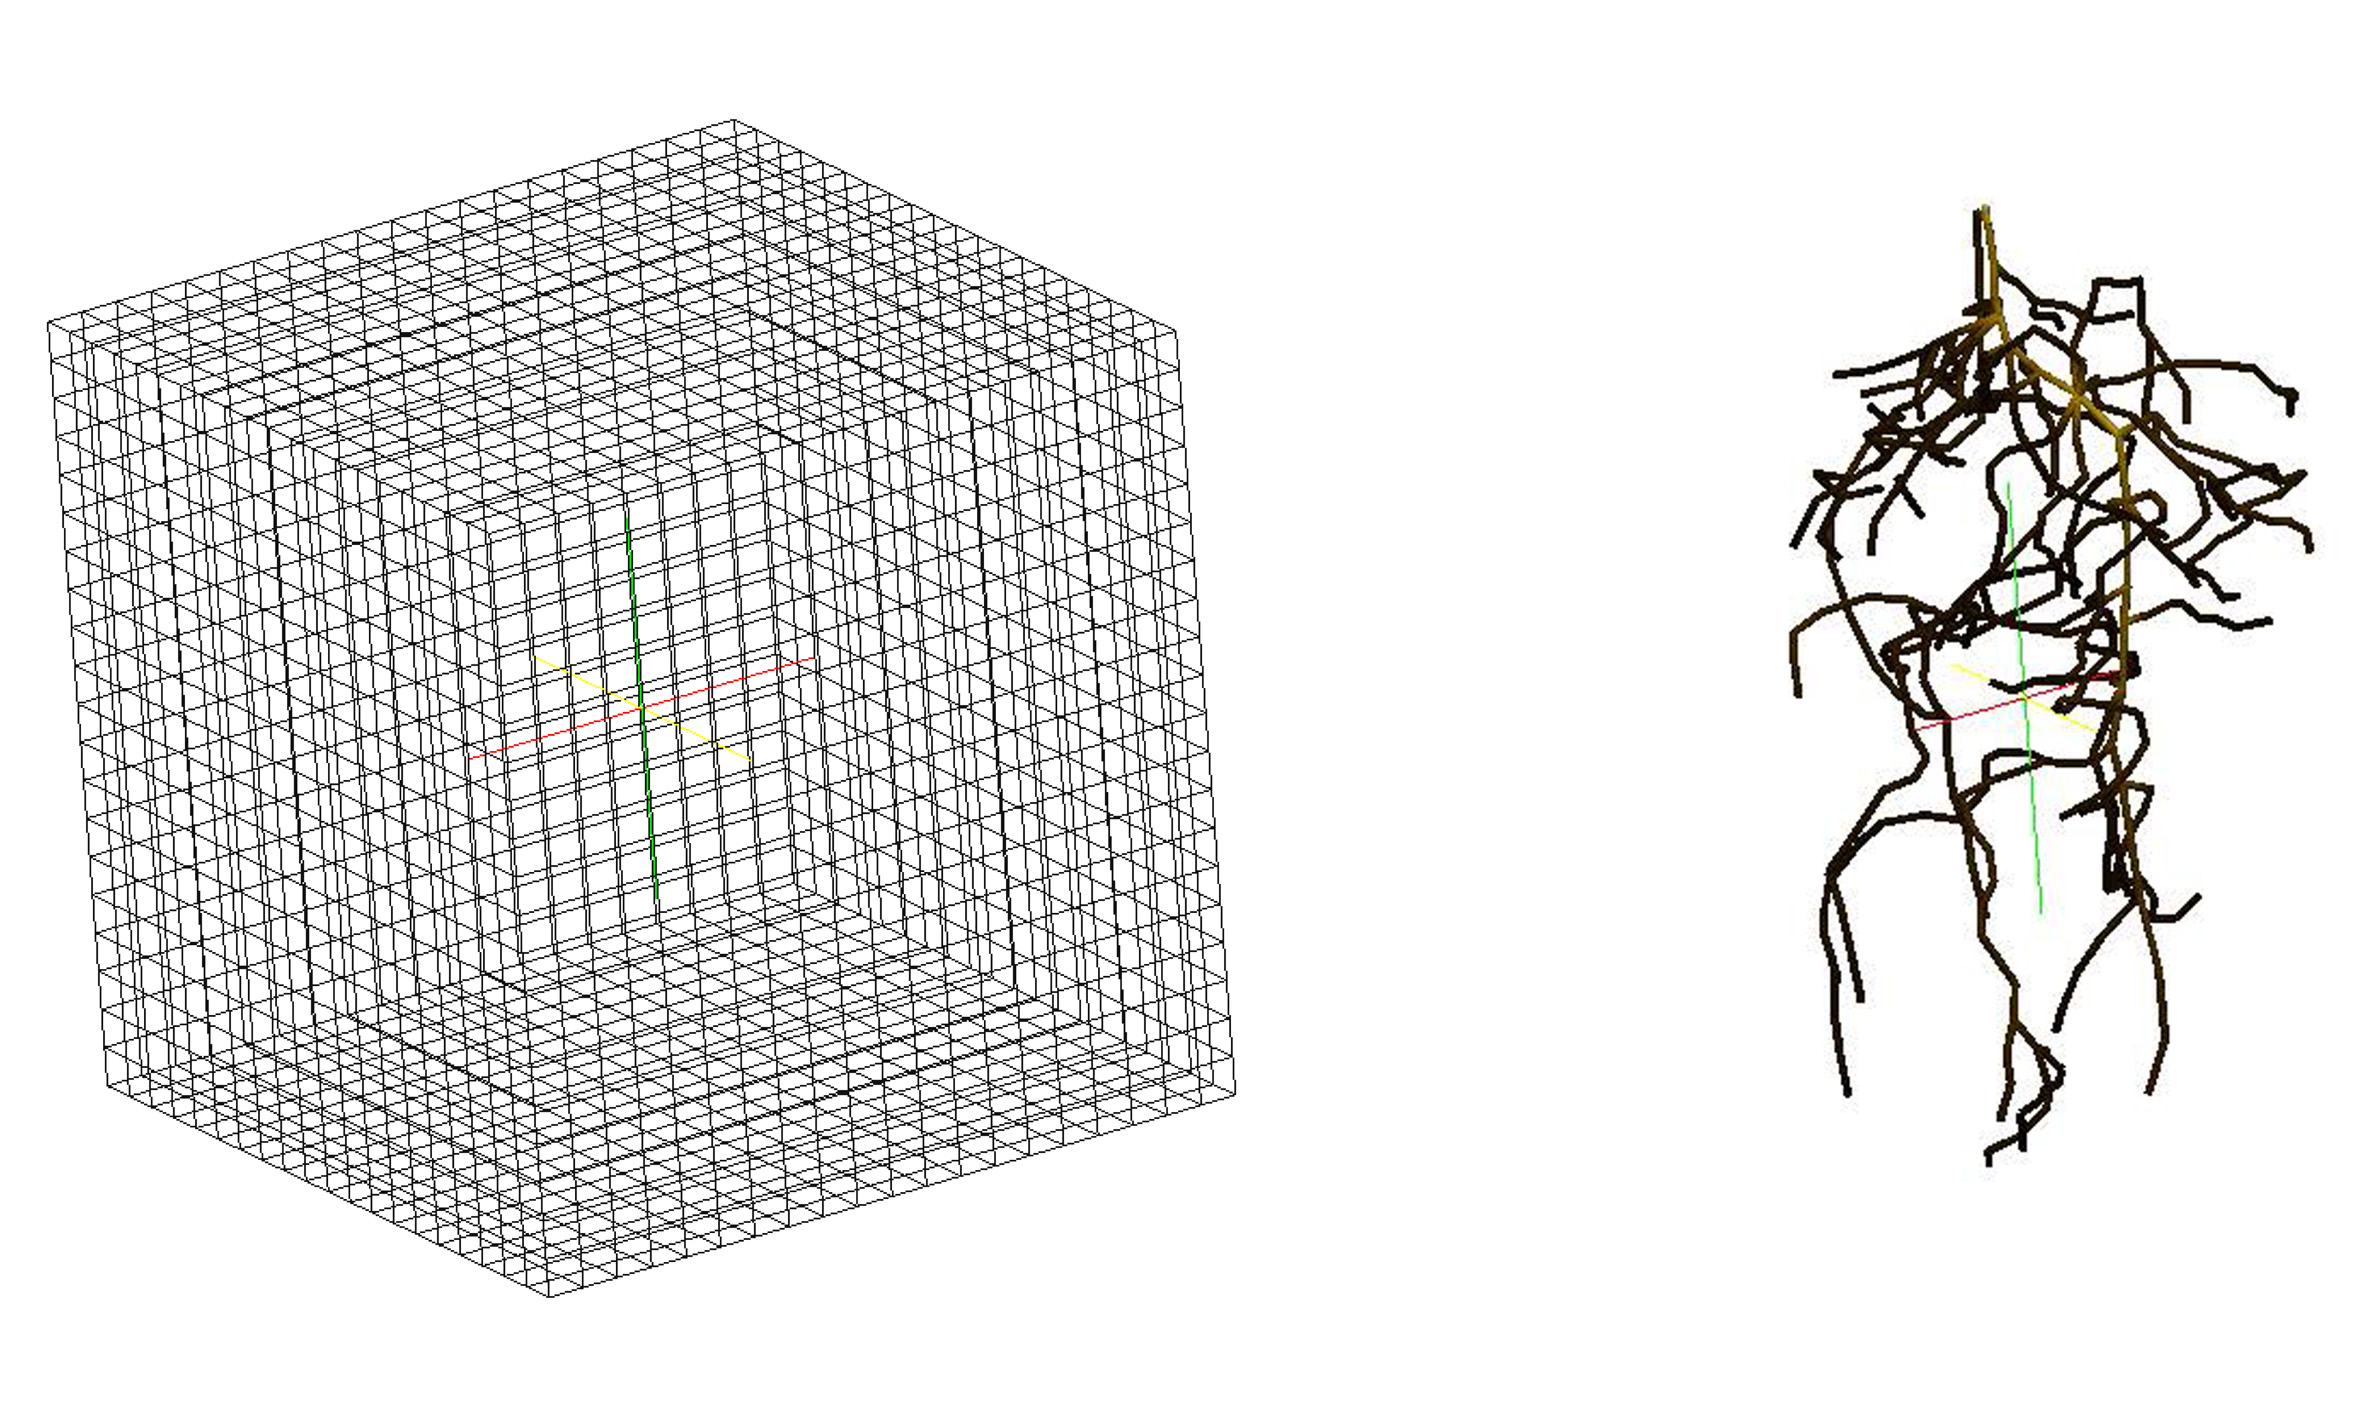
\includegraphics[width=0.5\textwidth]{grids.jpg}
	\caption{The 3D soil grid and the 1D, branched, grid representing the root architecture}
	\label{fig:grids}
\end{figure}

In the example of the coupled problems, both are used simultaneously. In that case, the two grids are merged via source/sink terms in positions where root and soil grids share the same spatial coordinates. This is illustrated in Fig. \ref{fig:merged}; detailed descriptions can be found in the individual examples. 
 
\begin{figure}[ht]
	\centering
  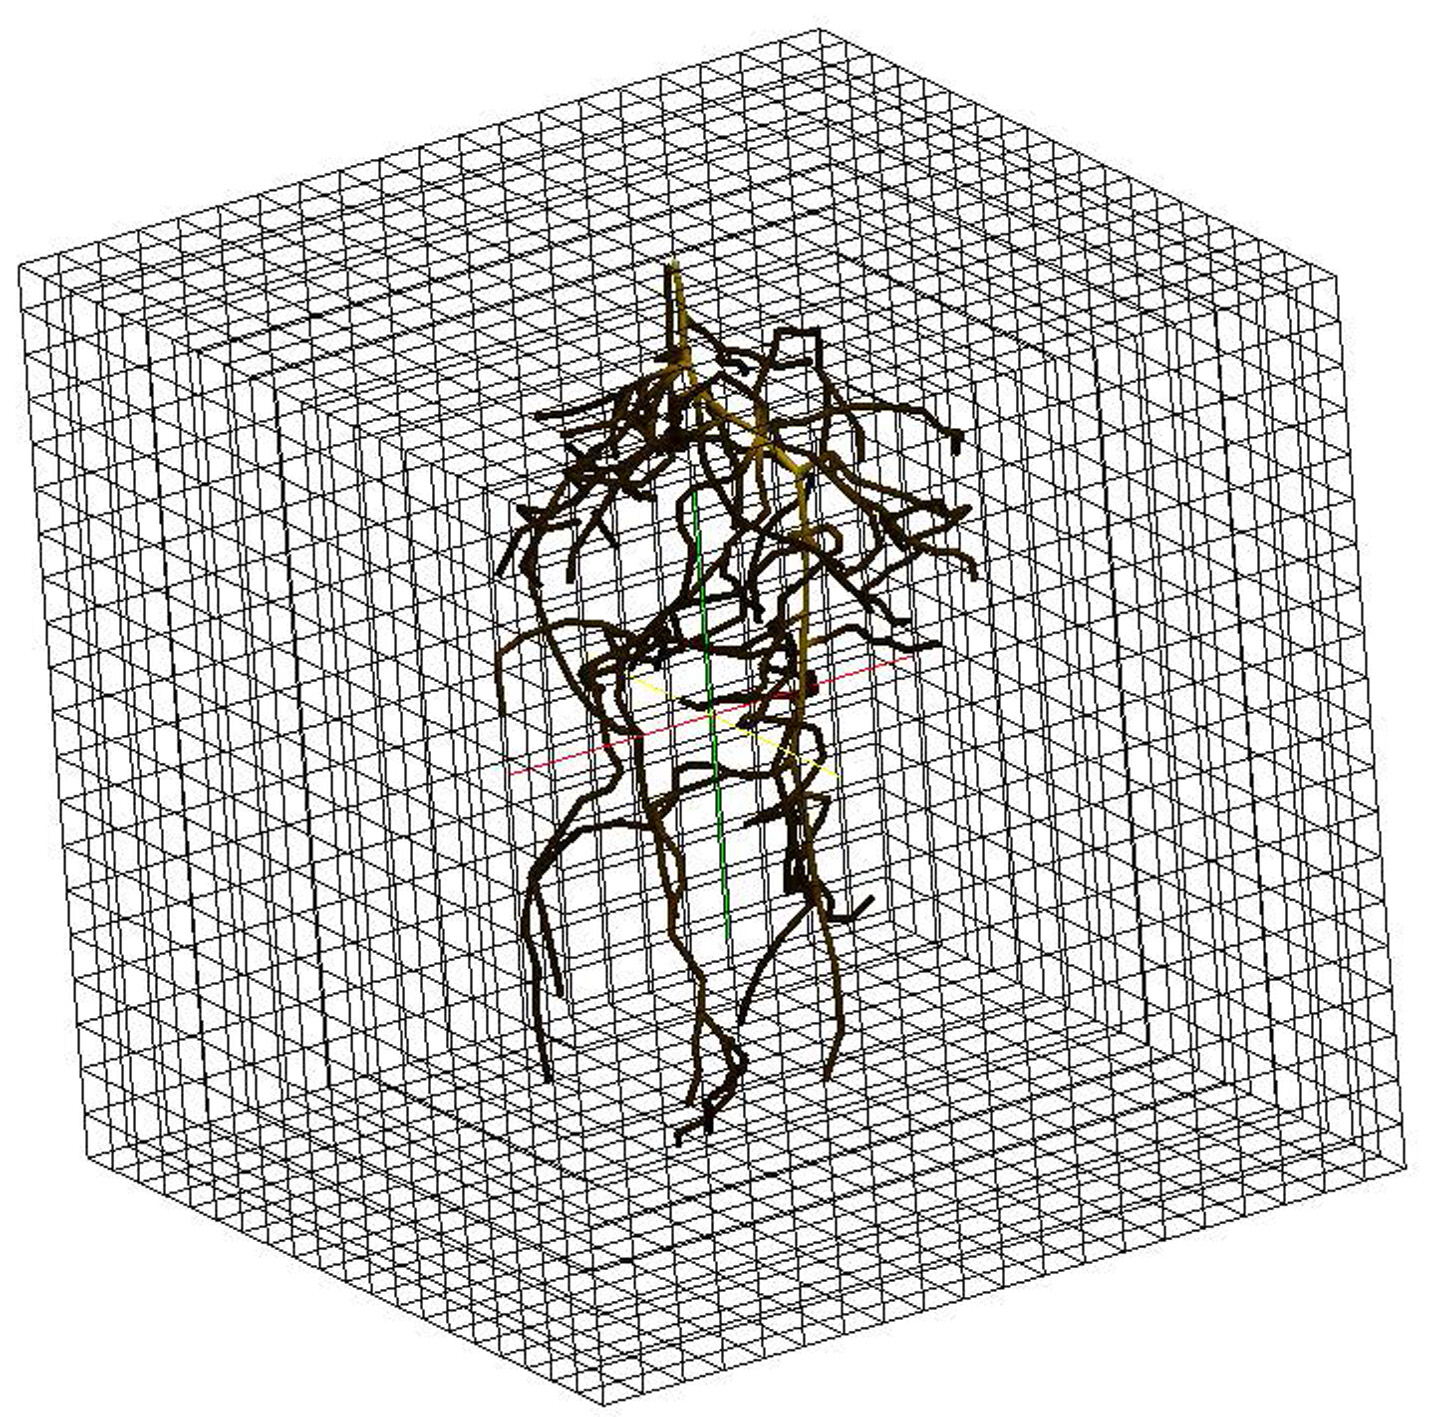
\includegraphics[width=0.33\textwidth]{merged.jpg}
	\caption{3D soil grid merged with the 1D, branched, grid representing the root architecture}
	\label{fig:merged}
\end{figure}

Grids can be created using different DUNE internal or external grid managers (see documentation of dune-grid). In the input file, the details about the numerical grids are specified in the groups [RootSystem.Grid] or [SoilGrid]. Each folder contains a folder named ``grids" where grids can be provided in dgf format. In the dumux-rosi examples, the soil grid is usually a structured grid created by the default ``GridCreator", where corner points of the domain, spatial resolution and cell type are specified such as in the following example: 

\begin{lstlisting}
[ Grid ]
LowerLeft = 0 0 0
UpperRight = 1 1 1
Cells = 10 10 20
CellType = Cube # or Simplex
\end{lstlisting}

There are two options to specify the root system grid. The first option is to specify it as a file in dgf-format that specifies the coordinates and connection of nodes (verteces).  

\begin{lstlisting}
DGF
Vertex
0.050000 0.050000 -0.000000
0.050000 0.050000 -0.0250000
0.050000 0.050000 -0.05000
0.050000 0.050000 -0.075000
#
SIMPLEX 
parameters 10 
0 1 1 0 3.14159e-05 0.01 0.0005 0.00 0.0001 0.00001 21922.1 
1 2 1 0 2.51327e-05 0.008 0.0005 0.00 0.0001 0.00001 39940.5 
2 3 1 0 2.51327e-05 0.008 0.0005 0.00 0.0001 0.00001 58409.5 
3 4 1 0 2.51327e-05 0.008 0.0005 0.00 0.0001 0.00001 77352.1 
4 5 1 0 2.51327e-05 0.008 0.0005 0.00 0.0001 0.00001 96793.2 
5 6 1 0 2.51327e-05 0.008 0.0005 0.00 0.0001 0.00001 116760 
#
BOUNDARYDOMAIN
default 1
#
\end{lstlisting}

The paragraph ``SIMPLEX" specifies 10 parameters for each root segment: node1ID, node2ID, type, branchID, surfaceIdx, length, radiusIdx, massIdx, axialPermIdx, radialPermIdx, creationTimeId in SI units. 

Root systems in dgf format can be computed from measured root systems as well as with the root architecture model CRootBox. 

The second option is to provide the root architectural parameters in the input file such that the root architecture and related grid is computed by CRootBox while used as a DuMu$^x$ module. 

\begin{lstlisting}
[RootSystem.Grid]
File = Triticum_aestivum_a_Bingham_2011  
InitialT = 10 # days
\end{lstlisting}

Important to know: It is currently necessary to build the code either for option 1 or for option 2 (i.e., two executables can be built that need to be provided with the correct input at runtime). 

\chapter*{Python for pre- and postprocessing}
We created a python layer around CRootBox and dumux-rosi for pre- and postprocessing such that the model can be run without handling the C++ code once an executable is available. 

For that, each example folder contains a folder named ''python`` that includes several examples as well a folder that includes the corresponding input files. 

\section*{The pre-processing}
Here, the path to the executable and corresponding input files is provided and the simulation is started, like in this example: 
\begin{lstlisting}
# go to the right place
path = os.path.dirname(os.path.realpath(__file__))
os.chdir(path)
os.chdir("../../../build-cmake/rosi_benchmarking/soil")

# run dumux
os.system("./richards1d benchmarks_1d/b1a.input")
\end{lstlisting}

\subsection*{The input file}
Here is an example of an input file,\\
\verb+/dumux-rosi-master/rosi_benchmarking/soil/benchmarks_1d/b1a.input+:
\lstinputlisting[firstline=1,lastline=34, language=C++, caption=Example input file]{dumux-rosi-master/rosi_benchmarking/soil/benchmarks_1d/b1a.input}	\\

Todo: periodic boundary conditions

\section*{The post-processing}
3D simulation results are stored in form of vtk files. If not specified otherwise, vtk files are stored for the initial and the final time point of the simulation. Using the key word ``CheckTimes" under the category ``Time loop" in the input file, additional output times can be specified. Time series, such as transpiration flux or pressure at the root collar over time, are stored as txt files. At the moment, this is specified within the problem file of the C++ code, see for example\\
\verb+/dumux-rosi-master/rosi_benchmarking/rootsystem/rootsproblem.hh+:
\lstinputlisting[firstline=172,lastline=172, language=C++, caption=Transpiration output]{dumux-rosi-master/rosi_benchmarking/rootsystem/rootsproblem.hh}	 
and
\lstinputlisting[firstline=360,lastline=361, language=C++, caption=Transpiration output]{dumux-rosi-master/rosi_benchmarking/rootsystem/rootsproblem.hh}	  

Here, results are read and plotted or further analysed, like in the following example. 
Using the \lstinline{vtk_tools} is particularly helpful for creating 1D plots such as depth profiles or time series in Python rather than using Paraview (Paraview of course is helpful for 3D visualisation).  

\begin{lstlisting}
# Figure 2a
s_, p_, z1_ = read1D_vtp_data("benchmark1d_1a-00001.vtp", False)
h1_ = vg.pa2head(p_)
ax1.plot(h1_, z1_ * 100, "r+")

np.savetxt("dumux1d_b1", np.vstack((z1_, h1_, z2_, h2_, z3_, h3_)), delimiter = ",")
\end{lstlisting}

\chapter*{Benchmarking example 1: Water flow in soil}
Currently, benchmarks are developed to test dumux-rosi against analytical solutions and results of other numerical models. They are all described in Jupyter Notebooks at \lstinline{https://github.com/RSA-benchmarks/collaborative-comparison}. Here, we describe the DuMu$^x$-implementation of the 1D benchmarks of Vanderborght et al. (2005) for water flow in soil.

\section*{The model}
We solve the Richards equation for water flow in soil. Since DuMu$^x$ is developed for multi-phase flow in porous media, it uses units of absolute pressure of wetting and non-wetting phases. In the Richards equation, we assume that the non-wetting phase (air) does not change over time and has a constant pressure of 1.0 $\times$ 10$^5$ Pa. Thus, we need to solve only the equation for the wetting phase (water). We stick to the standard DuMu$^x$ units for pressure, although in soil physics, head units are more common, in order to avoid mistakes of e.g. unconsidered hard coded constants, etc. The Richards equation thus can be written as 

\begin{equation}
\frac{\partial}{\partial t} \left(\rho_w \Phi S \right) - \nabla  \cdot \left[\rho_w \frac{\kappa}{\mu}K \left(\nabla p_w-\rho_w \mathbf{g} \right) \right] = 0,
\end{equation}
with $t$ time, $\theta$ water content, $S$ saturation, $\Phi$ porosity, $S \phi = \theta$, $\rho_w$ water density, $K$ intrinsic permeability, $\mu$ dynamic viscosity, $\kappa$ relative permeability, $\mathbf{g}$ gravitational acceleration, $p_w$ absolute pressure of wetting phase (water)\footnote{$p_w$ is the absolute pressure. The matric pressure $p_m$ is defined as $p_m = p_w-p_a$, where $p_a$ is the air pressure, assumed to be constant and equal to 1.0 $\times$ 10$^5$ Pa in this Richards equation model. In order to have head units, we need to convert the water potential from energy per unit volume of water (pressure) to energy per unit weight, i.e., $h_m=\frac{p_m}{\rho_w \mathbf{g}}$}. $\theta$ and $h_m$ are related by the water retention curve: $\theta:= \theta(h)$ (e.g. van Genuchten model).

Different initial and boundary conditions can be prescribed via the input file. Boundary conditions have number codes following (previous versions of) Hydrus: \\
constantPressure = 1,\\
constantFlux = 2, \\
atmospheric = 4, \\
freeDrainage = 5.

\section*{The input files}
Model parameters, initial and boundary conditions can be specified via the input file such that no re-building of the code is required. 
Here is the listing of the input file \lstinline{dumux-rosi-master/rosi_benchmarking/soil/benchmarks_1d/b1a.input}: 
\lstinputlisting[language={}, caption=input file]{dumux-rosi-master/rosi_benchmarking/soil/benchmarks_1d/b1a.input}	

\section*{The DuMu$^x$ code representation of model equations}
In this section, we explain where the different terms of the model equations can be found in the DuMu$^x$ code, i.e., the storage, flux and sink terms. 
The storage term is defined in the file \\
\verb+/dumux/dumux/porousmediumflow/Richards/localresidual.hh+, and is computed as\\
\lstinputlisting[firstline=91,lastline=93, language=C++, caption=Storage term]{dumux/dumux/porousmediumflow/richards/localresidual.hh}		
In this example, there is no source or sink term. 


The flux term is hidden in deeper layers of the code as part of the numerical scheme. In order to see it, we have to find out the flux type of the problem in the file 
\verb+/dumux/dumux/porousmediumflow/richards/...+. In this example, the flux type is ''darcyslaw``. Its implementation can then be found in the folder \verb+/dumux/dumux/flux+, and is then different for the different numerical schemes (e.g. cell-centered finite volume scheme with two-point flux approximation (TPFA)). 

%The file \verb+fluxvariables.hh+ in the folder \verb+/dumux/dumux/porousmediumflow/richards/+ defines the volume flux variable for the Richards equation by setting the nonwetting phase flux variable to zero. 
%\lstinputlisting[firstline=50,lastline=70, language=C++, caption=flux term b]{dumux/dumux/porousmediumflow/Richards/implicit/fluxvariables.hh}	

%The  definition for the wetting phase (water) is given in\\
%\verb+dumux/dumux/porousmediumflow/implicit/darcyfluxvariables.hh+. \\
%\lstinputlisting[firstline=19,lastline=349, language=C++, caption=flux term c]{dumux/dumux/porousmediumflow/implicit/darcyfluxvariables.hh}	

%The sink term is defined in the file\\ 
%\verb+dumux-rosi/rosi_examples/richardsrootsystem/richardstestproblem.hh+.\\
%\lstinputlisting[firstline=245,lastline=265, language=C++, caption=sink term]{dumux-rosi/rosi_examples/richardsrootsystem/richardstestproblem.hh}	

The implementation of the boundary conditions specified in the input file are implemented in the file\\ 
\verb+ dumux-rosi-master/rosi_benchmarking/soil/richardsproblem.hh+.\\
\lstinputlisting[firstline=188,lastline=224, language=C++, caption=Boundary conditions]{dumux-rosi-master/rosi_benchmarking/soil/richardsproblem.hh},
%
\lstinputlisting[firstline=229,lastline=252, language=C++, caption=Boundary conditions]{dumux-rosi-master/rosi_benchmarking/soil/richardsproblem.hh}	
and
\lstinputlisting[firstline=257,lastline=334, language=C++, caption=Boundary conditions]{dumux-rosi-master/rosi_benchmarking/soil/richardsproblem.hh}.		
											

\section*{Results}
The vtk output of 3D simulations may be visualised using Paraview. In this case, we only have a 1D simulation, therefore, we do the visualisation after postprocessing in Python. 

\begin{figure}[ht]
	\centering
  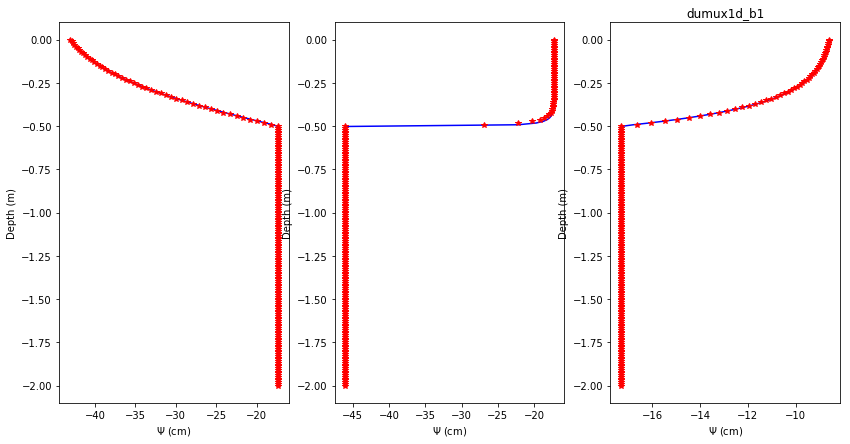
\includegraphics[width=1\textwidth]{benchmark1.png}
	\captionsetup{labelformat=empty}
	\caption{Results of benchmark problem 1. Blue: analytical solution, Red: numerical solution by DuMu$^x$}
	%\label{RWU}
\end{figure}



\end{document}
